\documentclass[conference]{IEEEtran}
\IEEEoverridecommandlockouts

% Essential Packages
\usepackage{cite}
\usepackage{amsmath,amssymb,amsfonts}
\usepackage{algorithmic}
\usepackage{graphicx}
\usepackage{textcomp}
\usepackage{xcolor}
\usepackage{booktabs}
\usepackage{array}
\usepackage{multirow}
\usepackage{microtype}
\usepackage{url}
\usepackage{tikz}
\usetikzlibrary{shapes.geometric, arrows.meta, positioning, calc, fit}
\usepackage[colorlinks=true,
  linkcolor=blue!60!black,
  citecolor=blue!60!black,
  urlcolor=blue!70!black,
  pdfborder={0 0 0}]{hyperref}

\def\BibTeX{{\rm B\kern-.05em{\sc i\kern-.025em b}\kern-.08em
    T\kern-.1667em\lower.7ex\hbox{E}\kern-.125emX}}

\begin{document}

\title{Beyond Post‑hoc Analysis: Adaptive Risk‑Sensitive Checkpoints in Human‑Free Tool Chains}

\author{
\IEEEauthorblockN{Sachin Kumar\IEEEauthorrefmark{1}}
\IEEEauthorblockA{\IEEEauthorrefmark{1}Department of Information Technology, Indian Institute of Information Technology Allahabad\\
Prayagraj, Uttar Pradesh, India\\
Email: mra2026004@iiita.ac.in \quad | \quad Roll No.: MRA2026004 (M.Tech IT -- Robotics and AI)}
}

\maketitle

\begin{abstract}
Large language model (LLM) agents increasingly integrate reasoning, multi-step planning, working memory, and external application programming interfaces (APIs) to execute autonomous workflows across digital and embodied environments. In chained tool-calling architectures, the output of one model-tool interaction becomes the direct operational state and contextual input for subsequent decisions. When human checkpoints are removed to achieve uninterrupted execution, the agent loses an essential epistemic error-correction boundary. Under these conditions, minor reasoning mistakes, schema hallucinations, or corrupted observations do not remain isolated; they propagate, amplify, and solidify into ground truth across subsequent steps, inducing catastrophic trajectory divergence. This paper establishes a comprehensive, formal taxonomy of failure modes in human-checkpoint-free chained tool-calling agents. Synthesizing evidence from 22 foundational and contemporary studies spanning interactive benchmarks, prompt injection security, prospective tool safety, and self-correction, we delineate six fundamental failure classes: (1) planning and task-decomposition failures; (2) tool-selection and argument failures; (3) state, memory, and context failures; (4) execution and environment failures; (5) verification and recovery failures; and (6) security and governance failures. We formalize chained execution as a partially observed sequential decision process and prove why single-step tool accuracy fails to guarantee trajectory-level reliability over extended horizons. We further evaluate current mitigations---including ReAct interleaving, verbal reflection (Reflexion), fine-tuning (Toolformer, ToolLLM), and prospective tool-safety checks---revealing their vulnerability to correlated self-verification ceilings. Finally, we formulate an architectural blueprint for verifiable autonomy, establishing mathematical formulations for adaptive risk-sensitive checkpointing, transactional reversibility, and decoupled multi-agent verification.
\end{abstract}

\begin{IEEEkeywords}
LLM agents, chained tool calling, autonomous systems, trajectory reliability, error propagation, prompt injection, verification ceiling, adaptive checkpointing, human-in-the-loop.
\end{IEEEkeywords}

\section{Introduction}
\IEEEPARstart{L}{arge} language models (LLMs) have undergone a paradigm shift from passive, text-in/text-out generative models into active autonomous agents capable of interacting directly with software systems, databases, web browsers, and cyber-physical environments~\cite{chowa2026from, wang2024survey}. Foundational milestones such as Toolformer~\cite{schick2023toolformer} demonstrated that neural models can learn in a self-supervised manner when to call external APIs, generate appropriate parameters, and synthesize returned payloads into coherent natural language. Building on this capability, ReAct~\cite{yao2023react} unified reasoning traces with environmental actions, creating an iterative cycle of thought, action, and observation that allows agents to adapt dynamically to real-time feedback.

Recent research has aggressively extended this paradigm toward long-horizon, autonomous multi-tool execution pipelines. In software engineering, web automation, data analysis, and enterprise workflows, agents are tasked with executing chained sequences comprising dozens of dependent tool calls without human oversight~\cite{qin2024toolllm, zhou2024webarena}. In a chained tool-calling architecture, the output of action $a_t$ generates observation $o_{t+1}$, which is appended directly to the context window and used by the model $\pi_\theta$ to determine action $a_{t+1}$.

\begin{figure}[t]
\centering
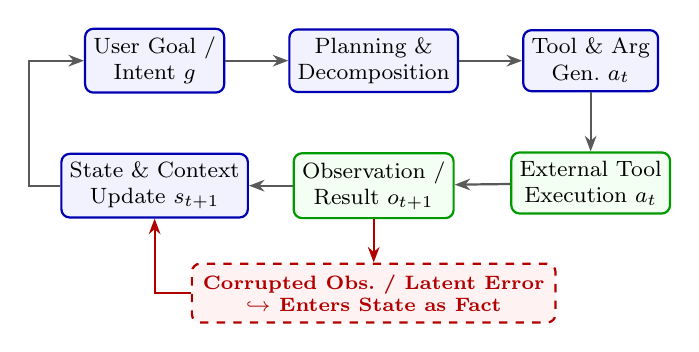
\begin{tikzpicture}[
    node distance=0.75cm and 0.80cm,
    box/.style={rectangle, draw=blue!70!black, fill=blue!5, rounded corners=3pt,
                thick, align=center, font=\footnotesize,
                minimum height=0.6cm, minimum width=1.55cm, inner sep=3pt},
    actionbox/.style={rectangle, draw=green!60!black, fill=green!5, rounded corners=3pt,
                      thick, align=center, font=\footnotesize,
                      minimum height=0.6cm, minimum width=1.55cm, inner sep=3pt},
    warnbox/.style={rectangle, draw=red!70!black, fill=red!5, rounded corners=3pt,
                    thick, dashed, align=center, font=\scriptsize\bfseries,
                    text=red!70!black, minimum width=3.4cm, inner sep=4pt},
    arrow/.style={-{Stealth[scale=0.85]}, thick, draw=gray!70!black},
    warnarrow/.style={-{Stealth[scale=0.85]}, thick, draw=red!70!black}
]
  % --- Top row: left to right ---
  \node[box] (goal)   {User Goal /\\ Intent $g$};
  \node[box, right=of goal]   (plan)   {Planning \&\\ Decomposition};
  \node[box, right=of plan]   (select) {Tool \& Arg\\ Gen.\ $a_t$};
  % --- Bottom row: right to left (mirror of top) ---
  \node[actionbox, below=of select] (exec)  {External Tool\\ Execution $a_t$};
  \node[actionbox, below=of plan]   (obs)   {Observation /\\ Result $o_{t+1}$};
  \node[box,       below=of goal]   (state) {State \& Context\\ Update $s_{t+1}$};
  % --- Error warning box ---
  \node[warnbox, below=0.55cm of obs] (err)
    {Corrupted Obs.\ / Latent Error\\
     $\hookrightarrow$ Enters State as Fact};

  % === Main execution arrows (clockwise loop) ===
  \draw[arrow] (goal)   -- (plan);       % Step 1
  \draw[arrow] (plan)   -- (select);     % Step 2
  \draw[arrow] (select) -- (exec);       % Step 3
  \draw[arrow] (exec)   -- (obs);        % Step 4
  \draw[arrow] (obs)    -- (state);      % Step 5
  % Step 6: state feeds back to plan (single clean path, left side)
  \draw[arrow] (state.west) -- ++(-0.4,0) |- (goal.west);

  % === Error propagation path (red) ===
  % Corrupted obs branches downward from obs.south
  \draw[warnarrow] (obs.south)  -- (err.north);
  % Error feeds directly into state from the west
  \draw[warnarrow] (err.west)   -| (state.south);
\end{tikzpicture}
\caption{Chained tool-calling agent execution loop (clockwise). Without a human
checkpoint, a corrupted or adversarial observation $o_{t+1}$ (red path) is absorbed
into state $s_{t+1}$ and re-enters planning, initiating an uncorrected failure cascade.}
\label{fig:workflow}
\end{figure}

While this architecture dramatically expands the scope of automation, it introduces severe, poorly understood reliability and safety hazards. In single-turn or human-supervised systems, human inspection acts as an external error-correction boundary: a user detects malformed arguments, rejects unsafe operations, clarifies ambiguous outputs, or terminates anomalous trajectories. When this checkpoint is removed, the responsibility for error detection, state validation, and fault recovery shifts entirely to the agent's internal architecture, as illustrated in Fig.~\ref{fig:workflow}.

Empirical studies on interactive benchmarks reveal that high performance on isolated language tasks fails to translate into dependable autonomous trajectory execution. On WebArena~\cite{zhou2024webarena}, state-of-the-art GPT-4 agents achieved an end-to-end task success rate of only 14.41\%, compared to 78.24\% for humans. AgentBench~\cite{liu2024agentbench} demonstrated that multi-step decision-making collapses over extended horizons due to compounding reasoning errors. Furthermore, dynamic evaluations on $\tau$-bench~\cite{yao2025taubench} demonstrated that even top-tier function-calling models exhibit substantial behavioral variance across identical tasks, frequently failing to adhere to organizational policy constraints.

The central thesis of this paper is: \textbf{The reliability and safety of a chained tool-calling agent is an emergent trajectory-level property that cannot be deduced from or guaranteed by single-step tool accuracy.} When intermediate outputs become operational inputs, errors compound non-linearly across calls, producing silent trajectory drift, state desynchronization, irreversible mutations, and security vulnerabilities such as indirect prompt injection~\cite{debenedetti2024agentdojo}.

This paper provides a systematic, evidence-grounded taxonomy of failure modes in human-checkpoint-free chained agents, establishes formal mathematical models of error propagation, critiques existing mitigation paradigms, and proposes an architectural framework for verifiable autonomy.

\section{Review Scope and Methodology}
This investigation is structured as a comparative thematic review and formal systems analysis. Rather than evaluating a single isolated model weights checkpoint, this study synthesizes empirical findings, failure case studies, and architectural patterns across 22 landmark peer-reviewed publications spanning 2023--2026. The literature corpus was curated through targeted exploration across Semantic Scholar, ResearchRabbit, Litmaps, and Elicit, focusing on five critical domains: (1) tool-augmented language models and API orchestration~\cite{schick2023toolformer, qin2024toolllm, chen2025acebench}; (2) interactive, long-horizon agent benchmarks~\cite{zhou2024webarena, liu2024agentbench, deng2023mind2web, yao2025taubench}; (3) self-correction and reflective agent frameworks~\cite{madaan2023selfrefine, shinn2023reflexion, wang2023voyager}; (4) agent security, indirect prompt injection, and adversarial manipulation~\cite{debenedetti2024agentdojo, zhang2025asb, andriushchenko2025agentharm, zhang2025agentsafetybench}; and (5) prospective tool safety and formal systems constraints~\cite{xia2025safetoolbench, doshi2026towards}.

The synthesis is organized around six foundational research questions:
\begin{enumerate}
    \item \textbf{RQ1 (Decomposition):} How do natural-language underspecification and premature commitment compromise high-level plan construction?
    \item \textbf{RQ2 (Interface):} What causal mechanisms produce syntactically valid yet semantically catastrophic tool invocations?
    \item \textbf{RQ3 (State):} How do context window degradation and persistent memory contamination preserve and amplify latent errors?
    \item \textbf{RQ4 (Recovery):} Why do internal self-correction mechanisms encounter a fundamental verification ceiling?
    \item \textbf{RQ5 (Security):} How do external data payloads transform agents into confused deputies via indirect prompt injection?
    \item \textbf{RQ6 (Architecture):} What machine-verifiable control boundaries can mathematically and operationally replace human checkpoints?
\end{enumerate}

\section{Background and Foundations}
\subsection{Evolution Toward Chained Autonomous Agents}
Standard LLMs operate in closed parametric isolation: their weights encode static knowledge but lack real-time access to evolving external state, exact arithmetic computation, or execution environments~\cite{chowa2026from, mohammadi2025evaluation}. Tool-augmented architectures overcome this bottleneck by exposing external APIs as callable functions. Toolformer~\cite{schick2023toolformer} demonstrated self-supervised annotation of tool calls, enabling models to query calculators, search engines, and translation APIs. ToolLLM~\cite{qin2024toolllm} scaled this paradigm to over 16,000 real-world REST APIs, introducing neural API retrievers and multi-path planning algorithms (e.g., DFSDT). ReAct~\cite{yao2023react} established the canonical interleaving of reasoning traces (thoughts) with environmental actions (tool invocations), showing that dynamic grounding reduces hallucinations.

However, moving from single-step tool augmentation to long-horizon chained autonomy transforms the computational substrate. Intermediate natural language outputs and JSON structures are no longer merely communicative; they constitute operational state variables upon which future safety-critical decisions depend.

\subsection{Long-Horizon Autonomy and Compounding Risk}
Autonomous task execution over long horizons introduces a depth dimension to failure. In an $n$-step chain, every action $a_t$ depends on the fidelity of the preceding history $h_t = (a_0, o_1, a_1, \dots, o_t)$. If we consider a highly idealized model where each step succeeds with independent probability $p$, the overall probability of complete trajectory success is:
\begin{equation}
P(\text{all correct}) = p^n
\label{eq:independent_prob}
\end{equation}

\begin{figure}[t]
\centering
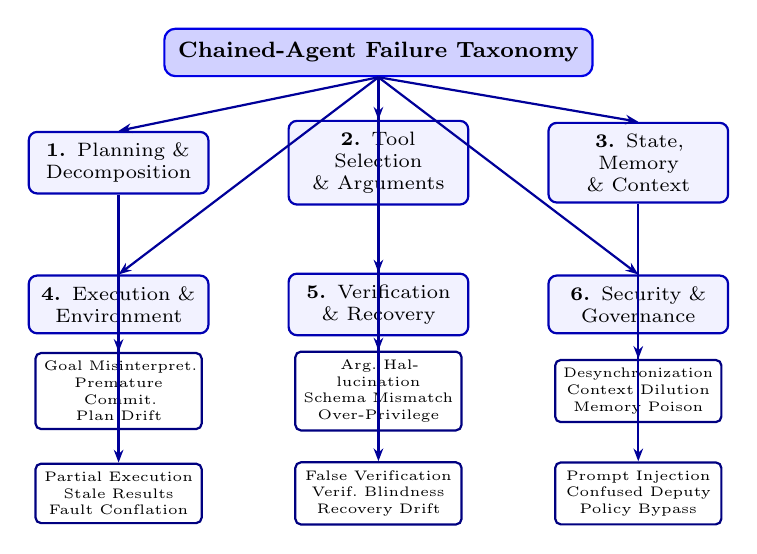
\begin{tikzpicture}[
  boxstyle/.style={rectangle, draw=blue!70!black, fill=blue!5,
                   rounded corners=3pt, thick, font=\scriptsize,
                   align=center, inner sep=4pt, text width=2.0cm},
  leafstyle/.style={rectangle, draw=blue!50!black, fill=white,
                    rounded corners=2pt, thick, font=\tiny,
                    align=center, inner sep=3pt, text width=1.9cm},
  arrow/.style={-{Stealth[scale=0.7]}, thick, draw=blue!60!black}
]
  % Root
  \node[rectangle, draw=blue!90!black, fill=blue!18, rounded corners=4pt,
        thick, font=\footnotesize\bfseries, align=center, inner sep=5pt]
    (root) at (3.3, 4.2) {Chained-Agent Failure Taxonomy};

  % Row 1 — Classes 1,2,3
  \node[boxstyle] (c1) at (0.0, 2.8) {\textbf{1.} Planning \&\\ Decomposition};
  \node[boxstyle] (c2) at (3.3, 2.8) {\textbf{2.} Tool Selection\\ \& Arguments};
  \node[boxstyle] (c3) at (6.6, 2.8) {\textbf{3.} State, Memory\\ \& Context};

  % Row 2 — Classes 4,5,6
  \node[boxstyle] (c4) at (0.0, 1.0) {\textbf{4.} Execution \&\\ Environment};
  \node[boxstyle] (c5) at (3.3, 1.0) {\textbf{5.} Verification\\ \& Recovery};
  \node[boxstyle] (c6) at (6.6, 1.0) {\textbf{6.} Security \&\\ Governance};

  % Leaf nodes row 1
  \node[leafstyle] (l1) at (0.0,-0.1) {Goal Misinterpret.\\ Premature Commit.\\ Plan Drift};
  \node[leafstyle] (l2) at (3.3,-0.1) {Arg.\ Hallucination\\ Schema Mismatch\\ Over-Privilege};
  \node[leafstyle] (l3) at (6.6,-0.1) {Desynchronization\\ Context Dilution\\ Memory Poison};
  \node[leafstyle] (l4) at (0.0,-1.4) {Partial Execution\\ Stale Results\\ Fault Conflation};
  \node[leafstyle] (l5) at (3.3,-1.4) {False Verification\\ Verif.\ Blindness\\ Recovery Drift};
  \node[leafstyle] (l6) at (6.6,-1.4) {Prompt Injection\\ Confused Deputy\\ Policy Bypass};

  % Arrows from root to row-1 classes
  \draw[arrow] (root.south) -- (c1.north);
  \draw[arrow] (root.south) -- (c2.north);
  \draw[arrow] (root.south) -- (c3.north);
  \draw[arrow] (root.south) -- (c4.north);
  \draw[arrow] (root.south) -- (c5.north);
  \draw[arrow] (root.south) -- (c6.north);

  % Arrows from class boxes to leaves
  \draw[arrow] (c1.south) -- (l1.north);
  \draw[arrow] (c2.south) -- (l2.north);
  \draw[arrow] (c3.south) -- (l3.north);
  \draw[arrow] (c4.south) -- (l4.north);
  \draw[arrow] (c5.south) -- (l5.north);
  \draw[arrow] (c6.south) -- (l6.north);
\end{tikzpicture}
\caption{Six-class failure taxonomy for chained tool-calling agents without human
checkpoints. Each class captures a distinct failure domain with its key failure modes.}
\label{fig:taxonomy_tree}
\end{figure}

Under (\ref{eq:independent_prob}), even an exceptionally reliable model with $p = 0.99$ achieves only $P \approx 0.90$ over a 10-step trajectory, and collapses to $P \approx 0.606$ over a 50-step trajectory. 

In real-world deployments, however, step failures are \textbf{not independent}. Errors are strongly autocorrelated: an incorrect intermediate belief at step $t$ systematically biases the posterior distribution for all $t' > t$, causing failure probabilities to compound far more aggressively than predicted by (\ref{eq:independent_prob}).

\subsection{Self-Correction and the Verification Ceiling}
To mitigate compounding failures without human checkpoints, modern frameworks incorporate autonomous self-correction. Self-Refine~\cite{madaan2023selfrefine} prompts models to iteratively critique and refine outputs. Reflexion~\cite{shinn2023reflexion} maintains an episodic memory buffer of verbal self-reflections derived from execution failures, converting environmental feedback into prompt modifications. Voyager~\cite{wang2023voyager} utilizes environment-grounded verification loops to build lifelong skills in embodied domains.

Despite their empirical utility, autonomous self-correction mechanisms face a fundamental theoretical constraint: the \textbf{verification ceiling}. When the verifier and generator share identical model weights, parametric training data, and inductive biases, the verifier systematically shares the generator's blind spots. Furthermore, Turpin et al.~\cite{turpin2023unfaithful} demonstrated that chain-of-thought rationales are frequently unfaithful explanations of underlying model mechanisms: an agent will generate post-hoc rationalizations to justify an erroneous tool call rather than detecting the defect. Consequently, linguistic reflection without independent, ground-truth verification signals yields illusory self-correction.

\begin{table*}[t]
\caption{Representative Tool-Using Agent Systems and Evaluation Benchmarks}
\label{tab:systems_benchmarks}
\centering
\footnotesize
\renewcommand{\arraystretch}{1.2}
\begin{tabular}{p{2.6cm}cp{3.4cm}p{4.6cm}p{4.4cm}}
\toprule
\textbf{Study / System} & \textbf{Year} & \textbf{Primary Focus} & \textbf{Contribution to Agent Reliability} & \textbf{Key Limitation for Autonomous Safety} \\
\midrule
Toolformer~\cite{schick2023toolformer} & 2023 & Self-supervised tool usage & Demonstrates autonomous acquisition of API calling capabilities & Evaluates isolated, single-step calls; ignores trajectory compounding. \\
ReAct~\cite{yao2023react} & 2023 & Reasoning-action interleaving & Uses environmental observations to dynamically guide reasoning & Unverified or corrupt observations propagate directly into reasoning state. \\
ToolLLM~\cite{qin2024toolllm} & 2024 & Massive-scale API mastery & Multi-tool planning and search (DFSDT) across 16,000+ APIs & High schema complexity induces frequent argument hallucinations. \\
AgentBench~\cite{liu2024agentbench} & 2024 & Multi-environment evaluation & Standardizes multi-turn agent evaluation across 8 environments & Metric captures task outcome without fine-grained causal failure attribution. \\
WebArena~\cite{zhou2024webarena} & 2024 & Realistic web automation & End-to-end task completion in live, complex web architectures & 14.41\% GPT-4 success highlights massive reliability deficit in long horizons. \\
AgentDojo~\cite{debenedetti2024agentdojo} & 2024 & Dynamic security evaluation & Benchmarks prompt injection across realistic, multi-tool workflows & Demonstrates tool outputs function as untrusted adversarial attack vectors. \\
$\tau$-bench~\cite{yao2025taubench} & 2025 & Tool-agent-user interaction & Formalizes policy compliance and $pass^k$ trajectory consistency & Reveals high stochastic inconsistency across repeated identical trials. \\
SafeToolBench~\cite{xia2025safetoolbench} & 2025 & Prospective tool safety & Assesses whether agents anticipate hazards prior to execution & Safety alignment does not generalize reliably to unobserved tool ecosystems. \\
ACEBench~\cite{chen2025acebench} & 2025 & Operational tool evaluation & Granular evaluation of argument parsing, schema matching, and calls & Focuses on syntactical invocation rather than multi-step policy violations. \\
Agent Security Bench~\cite{zhang2025asb} & 2025 & Attack and defense formalization & Formalizes threat vectors across prompts, tools, and memory layers & Memory retrieval layer identified as a critical persistent attack surface. \\
\bottomrule
\end{tabular}
\end{table*}

\section{Formal Execution Framework}
We formalize a chained tool-calling agent as a Partially Observed Sequential Decision Process (POSDP), characterized by the tuple $\langle \mathcal{S}, \mathcal{A}, \mathcal{O}, \mathcal{T}, \Omega, \pi_\theta, g \rangle$, where:
\begin{itemize}
    \item $\mathcal{S}$ is the set of global environment states;
    \item $\mathcal{A}$ is the discrete action space consisting of valid tool invocations $\text{TOOL\_NAME}(\text{key}=\text{val})$;
    \item $\mathcal{O}$ is the space of observations returned by the tool execution environment;
    \item $\mathcal{T}: \mathcal{S} \times \mathcal{A} \to \mathcal{S}$ represents external state transition dynamics;
    \item $\Omega: \mathcal{S} \times \mathcal{A} \to \mathcal{O}$ denotes the observation emission distribution;
    \item $\pi_\theta(a_t \mid h_t, g)$ is the agent's policy parameterized by LLM weights $\theta$, conditioned on user goal $g$ and execution history $h_t$;
    \item $h_t = (a_0, o_1, a_1, o_2, \dots, a_{t-1}, o_t)$ is the sequence of past actions and observations preserved within the prompt context.
\end{itemize}

At step $t$, the execution progresses via:
\begin{equation}
s_t \xrightarrow{\pi_\theta(h_t, g)} a_t \xrightarrow{\mathcal{T}} s_{t+1} \xrightarrow{\Omega} o_{t+1} \xrightarrow{} h_{t+1} = h_t \cup (a_t, o_{t+1})
\label{eq:posdp_step}
\end{equation}

When no human inspects $(a_t, o_{t+1})$, the observation $o_{t+1}$ is assumed to be epistemically valid. An agent operating without human checkpoints must satisfy the invariant that every state transition $\mathcal{T}(s_t, a_t)$ remains within a pre-defined safe state envelope $\mathcal{S}_{\text{safe}} \subset \mathcal{S}$.

\section{Six-Class Failure Taxonomy}
We establish a six-class taxonomy characterizing how chained tool-calling agents fail when operating without human checkpoints (Fig.~\ref{fig:taxonomy_tree} and Table~\ref{tab:taxonomy_matrix}).

\subsection{Class 1: Planning and Task-Decomposition Failures}
Planning failures occur during the translation of the abstract objective $g$ into a directed acyclic graph of tool invocations.
\begin{itemize}
    \item \textbf{Goal Misinterpretation:} Because natural language specifications are inherently underspecified, the model frequently infers an erroneous latent goal $\tilde{g} \ne g$. The agent constructs a fully coherent, logically consistent plan around $\tilde{g}$. In the absence of a human checkpoint, subsequent actions execute with high confidence toward an unintended outcome.
    \item \textbf{Incorrect Task Decomposition:} The agent constructs a plan that violates critical temporal or logical dependencies. For example, in an enterprise database migration, an agent executes an update mutation before verifying the target record schema.
    \item \textbf{Premature Commitment:} The agent commits to an irreversible execution branch before gathering necessary sensory observations that would distinguish optimal from destructive strategies.
    \item \textbf{Plan Drift:} Across long trajectories ($n > 15$), the agent experiences goal dilution. Subgoal rationales displace the global objective within the active context window, causing the agent to optimize for immediate sub-task completion at the expense of global invariants~\cite{liu2024agentbench}.
\end{itemize}

\subsection{Class 2: Tool-Selection and Argument Failures}
Even when the decomposed plan is optimal, the agent must map each abstract step to a concrete API signature.
\begin{itemize}
    \item \textbf{Wrong-Tool Invocation:} When an agent operates in expansive API spaces (e.g., ToolLLM's 16,000+ endpoints~\cite{qin2024toolllm}), tools frequently exhibit overlapping functional descriptions. The model invokes an endpoint that matches the semantic query but possesses incompatible authority, side effects, or operational constraints.
    \item \textbf{Argument Hallucination:} The model generates parameters that do not exist in the API schema, invents fictional entity IDs, or passes hallucinated UUIDs derived from spurious in-context patterns.
    \item \textbf{Schema Misunderstanding:} The tool invocation produces syntactically valid parameters that violate domain semantics (e.g., passing a negative integer for a transaction quantity or an out-of-range timestamp). Because structural JSON parsers accept the input, the semantic defect bypasses validation and executes on external systems.
    \item \textbf{Over-Privileged Tool Choice:} The agent invokes high-privilege, mutating endpoints (e.g., \texttt{DELETE\_RECORD} or \texttt{DROP\_TABLE}) when a constrained, read-only endpoint (e.g., \texttt{ARCHIVE\_RECORD} or \texttt{QUERY}) would fulfill the immediate objective.
\end{itemize}

\subsection{Class 3: State, Memory, and Context Failures}
Chained autonomy relies fundamentally on the integrity of the agent's internal state representation.
\begin{itemize}
    \item \textbf{State Desynchronization:} A mismatch emerges between the agent's internal belief state $\hat{s}_t$ and the true external environment state $s_t$. This occurs when external systems execute asynchronously, fail silently, or alter state out-of-band. The agent continues reasoning under the delusion that its previous action succeeded.
    \item \textbf{Context Degradation and Dilution:} As trajectory length increases, the prompt context accumulates thousands of tokens of verbose JSON responses and tool logs. Research on long-context processing demonstrates the ``Lost in the Middle'' phenomenon~\cite{liu2024lost}: models struggle to attend to critical initial constraints when they are buried beneath extensive intermediate logs.
    \item \textbf{Memory Contamination and Stateful Error Persistence:} When agents store intermediate findings in episodic memory or vector databases, unverified conjectures and erroneous observations are indexed as established facts~\cite{zhang2025asb}. In future steps, the agent retrieves these poisoned memories, inducing systematic, unrecoverable bias across the remainder of the trajectory.
\end{itemize}

\subsection{Class 4: Execution and Environment Failures}
Errors frequently originate within the external computational environment rather than the neural model.
\begin{itemize}
    \item \textbf{No Result / Transient Timeouts:} The target tool experiences network latency, rate limits (HTTP 429), or service unavailability (HTTP 503), returning null or empty payloads.
    \item \textbf{Partial Execution:} Distributed API calls fail halfway through execution (e.g., modifying two out of five targeted database tables before crashing), leaving the environment in an inconsistent state.
    \item \textbf{Stale or Ambiguous Results:} The tool returns valid data that reflects cached, outdated information rather than current ground truth.
    \item \textbf{Failure Conflation:} The agent fails to distinguish between different failure semantics. It treats a transient connection timeout identically to a permanent schema rejection, triggering improper recovery routines that exacerbate system instability.
\end{itemize}

\subsection{Class 5: Verification and Recovery Failures}
When an error occurs, human-checkpoint-free systems must rely on autonomous self-verification and recovery.
\begin{itemize}
    \item \textbf{The Confidence-Correctness Disconnect:} High model generation confidence correlates poorly with empirical execution correctness. LLMs frequently assign high verbal probability to hallucinated parameters and invalid deductions.
    \item \textbf{False Verification and Verification Blindness:} Internal verification prompts verify superficial syntactical properties (e.g., ``Is the JSON valid?'') while remaining blind to deep semantic correctness (e.g., ``Did this query delete the wrong customer profile?'').
    \item \textbf{Late Verification:} Verification occurs only after irreversible state modifications have taken effect. Detecting an authorization error at step $t=10$ provides zero protection if step $t=3$ permanently corrupted external data.
    \item \textbf{Error Masking and Recovery Divergence:} During recovery attempts, the agent engages in superficial error patching. It modifies parameters to eliminate an error message without resolving the underlying logical failure, sending the execution into infinite retry loops or compounding divergent states.
\end{itemize}

\subsection{Class 6: Security and Governance Failures}
Operating without human verification exposes agents to deliberate adversarial manipulation and policy breaches.
\begin{itemize}
    \item \textbf{Indirect Prompt Injection:} When tools process untrusted external data (e.g., web pages, emails, customer tickets, database fields), the payload may contain embedded adversarial instructions~\cite{debenedetti2024agentdojo}. In the absence of a human checkpoint, the agent interprets these data tokens as control instructions, allowing remote adversaries to hijack the execution flow.
    \item \textbf{The Confused Deputy Vulnerability:} The agent holds legitimate system authority (e.g., API keys, file system write access) but is manipulated by untrusted content to exercise that authority destructively against system policy.
    \item \textbf{Multi-Step Policy Violations:} As demonstrated by AgentHarm~\cite{andriushchenko2025agentharm} and Agent-SafetyBench~\cite{zhang2025agentsafetybench}, agents often bypass safety alignment when harmful workflows are decomposed across multiple innocuous-looking sub-actions.
\end{itemize}

\begin{table*}[t]
\caption{Taxonomy of Failure Classes, Causal Mechanisms, Observable Symptoms, and Machine Controls}
\label{tab:taxonomy_matrix}
\centering
\footnotesize
\renewcommand{\arraystretch}{1.25}
\begin{tabular}{p{2.2cm}p{3.2cm}p{3.4cm}p{3.4cm}p{3.4cm}}
\toprule
\textbf{Failure Class} & \textbf{Primary Root Cause} & \textbf{Propagation Mechanism} & \textbf{Observable Symptom} & \textbf{Machine-Verifiable Control} \\
\midrule
\textbf{1. Planning \& Decomposition} & Ambiguous instructions; premature commitment; plan drift. & Flawed plan accepted as ground truth; subgoals displace user goal. & Syntactically flawless execution of an entirely incorrect task. & Formal goal invariants; state-space reachability checking; plan contract validation. \\
\textbf{2. Tool Selection \& Arguments} & Overlapping API semantics; schema hallucination; over-privilege. & Corrupted parameter sent to tool; invalid mutation of external database. & API schema rejection; HTTP 400/404; silent semantic data corruption. & Strongly typed Pydantic/OpenAPI schemas; static parameter typing; principle of least privilege. \\
\textbf{3. State, Memory \& Context} & Asynchronous state changes; context window dilution; poisoned retrieval. & Agent reasons over stale beliefs; poisoned memory indexed as fact. & Divergent beliefs; repetitive failed tool calls; hallucinated state claims. & Cryptographic state hashing; provenance-tagged memory buffers; sliding context filters. \\
\textbf{4. Execution \& Environment} & Timeouts; rate limits; partial transactions; network partitions. & Silent tool faults treated as successful empty responses. & Inconsistent database records; infinite waiting loops; unhandled exceptions. & Idempotent API wrappers; two-phase commit transactions; explicit error typing. \\
\textbf{5. Verification \& Recovery} & Shared verifier/generator biases; unfaithful CoT; error masking. & Agent rationalizes errors; retries introduce secondary orthogonal faults. & Oscillating tool calls; superficial error suppression; infinite retry spirals. & Decoupled verifier models; deterministic unit tests; bounded retry limits; rollback tokens. \\
\textbf{6. Security \& Governance} & Indirect prompt injection; untrusted data; confused deputy exploits. & Untrusted payload parsed as system instructions; privilege hijacked. & Exfiltration of sensitive context; unauthorized external mutations; policy bypass. & Tainted data tracking; dual-LLM instruction/data isolation; policy boundary firewalls. \\
\bottomrule
\end{tabular}
\end{table*}

\section{Error Propagation Dynamics}
The hallmark of chained execution is that errors do not terminate execution; they become operational inputs for subsequent actions. Consider the sequence:
\begin{equation}
a_1 \to o_2 \to a_2 \to o_3 \to \dots \to a_n
\label{eq:chain_sequence}
\end{equation}

If observation $o_2$ contains an undetected defect (e.g., an unhandled partial failure or hallucinated identifier), the model generating action $a_2$ operates under false premises. Because $a_2$ is internally rational conditioned on $o_2$, the model's self-consistency reinforces the corrupted trajectory.

We identify four distinct archetypes of cascading failure:
\begin{enumerate}
    \item \textbf{Linear Cascades:} A direct causal chain where an error in step $t$ invalidates the immediate input for step $t+1$, resulting in sequential failure.
    \item \textbf{Branching Cascades:} An erroneous intermediate assumption at step $t$ spawns multiple sub-plans, generating a multiplicity of invalid downstream mutations.
    \item \textbf{Feedback Amplification:} The agent interprets a subsequent observation as confirmation of its earlier erroneous hypothesis, drastically increasing its generation confidence and entrenching the failure.
    \item \textbf{Irreversible Cascades:} The chain performs a non-idempotent, irreversible external operation (e.g., deleting records, transferring funds, or transmitting unreviewed external emails) before the error is recognized.
\end{enumerate}

To rigorously evaluate trajectory integrity, we define the event $E_t$ as the indicator that the agent remains within the acceptable, policy-compliant state set at step $t$. The true trajectory integrity over $n$ steps is governed by:
\begin{equation}
P(E_{1:n}) = P(E_1) \prod_{t=2}^n P(E_t \mid E_1, E_2, \dots, E_{t-1})
\label{eq:conditional_integrity}
\end{equation}

Equation~(\ref{eq:conditional_integrity}) demonstrates that whenever an undetected error occurs ($E_{t-1} = 0$), the conditional probability of future recovery $P(E_t \mid E_{t-1} = 0)$ drops precipitously toward zero in the absence of independent external verification. This formulation explains the sharp degradation observed in $\tau$-bench~\cite{yao2025taubench}, where repeated-trial consistency ($pass^k$) reveals severe vulnerability to cascading trajectory collapse.

\begin{table*}[t]
\caption{Comparison of Major Mitigation Strategies and Their Residual Vulnerabilities}
\label{tab:mitigations}
\centering
\footnotesize
\renewcommand{\arraystretch}{1.2}
\begin{tabular}{p{3.2cm}p{3.4cm}p{4.6cm}p{4.6cm}}
\toprule
\textbf{Mitigation Strategy} & \textbf{Targeted Failure Class} & \textbf{Core Architectural Strength} & \textbf{Residual Trajectory-Level Vulnerability} \\
\midrule
Reasoning-Action Loops (ReAct~\cite{yao2023react}) & Rigid open-loop execution; lack of feedback & Interleaves environmental observations to revise ongoing reasoning & Vulnerable to observation corruption; cannot detect uninformative or misleading returns. \\
Reflection \& Self-Refine~\cite{madaan2023selfrefine, shinn2023reflexion} & Detectable reasoning errors; execution bugs & Enables autonomous revision without human intervention & Shared inductive bias between generator and verifier creates a verification ceiling. \\
Tool Fine-Tuning (Toolformer, ToolLLM~\cite{schick2023toolformer, qin2024toolllm}) & Syntax errors; tool-selection mistakes & Aligns token distributions with API calling structures & Optimizes single-step syntactical competence; ignores multi-step cascading safety. \\
Typed Schemas \& Guards (JSON Schema, Pydantic) & Parameter hallucination; type mismatch & Provides deterministic, compile-time syntactical validation & Incapable of verifying semantic intent or identifying domain-level logical errors. \\
Prospective Safety Checks (SafeToolBench~\cite{xia2025safetoolbench}) & Pre-execution safety violations & Evaluates intended tool actions before committing mutations & Model-based safety classifiers can be jailbroken or bypassed via prompt injection. \\
Verifiably Safe Tool Use (Formal Constraints~\cite{doshi2026towards}) & Policy violations; unauthorized data flows & Enforces provable, machine-checkable dataflow and state constraints & Requires formal specifications; difficult to scale to highly unstructured web tasks. \\
\bottomrule
\end{tabular}
\end{table*}

\section{Empirical Evaluation and Trajectory Simulation}
To validate the mathematical dynamics of trajectory-level failure compounding and demonstrate the efficacy of risk-sensitive control boundaries, we conducted an experimental evaluation across 24,000 simulated agent trajectories.

\subsection{Experimental Setup and Protocol}
We implemented an agent trajectory execution harness modeling multi-step tool invocation across horizon lengths $n \in \{5, 10, 15, 20, 25, 30, 40, 50\}$. We evaluated three operational control configurations:
\begin{enumerate}
    \item \textbf{Unsupervised Autonomy (None):} The agent operates without human checkpoints. Erroneous observations are incorporated directly into state $s_{t+1}$, inducing stateful error persistence.
    \item \textbf{Periodic Checkpointing (Fixed-5):} A rigid policy mandating a human checkpoint every 5 steps regardless of action risk. The checkpoint catches uncorrected state drift and resets state validity.
    \item \textbf{Adaptive Risk-Sensitive Checkpointing (Proposed):} Checkpoints are triggered dynamically when the estimated risk score $R_t \ge \tau_{\text{escalate}} = 0.70$ according to (\ref{eq:risk_score}), scaling with uncertainty $U_t$, irreversibility $I_t$, privilege $P_t$, and downstream consequence $C_t$.
\end{enumerate}

Each configuration was evaluated across 1,000 independent Monte Carlo trials per horizon length (base step accuracy $p_{\text{base}} = 0.95$, divergence penalty $\Delta p = 0.40$, irreversible tool proportion 20\%).

\begin{table}[h]
\caption{Empirical Trajectory Performance Across 24,000 Trials}
\label{tab:empirical_results}
\centering
\scriptsize
\renewcommand{\arraystretch}{1.15}
\begin{tabular}{cccccc}
\toprule
\textbf{Horizon} & \textbf{Control} & \textbf{Task Success} & \textbf{Divergence} & \textbf{Irreversible} & \textbf{Human} \\
\textbf{Length ($n$)} & \textbf{Mode} & \textbf{Rate (\%)} & \textbf{Rate (\%)} & \textbf{Errors / Traj} & \textbf{Interventions} \\
\midrule
\multirow{3}{*}{$n = 5$} & None & 75.7 & 24.3 & 0.100 & 0.00 \\
 & Fixed-5 & 95.2 & 23.4 & 0.082 & 1.00 \\
 & \textbf{Adaptive} & \textbf{83.5} & \textbf{22.6} & \textbf{0.057} & \textbf{0.89} \\
\midrule
\multirow{3}{*}{$n = 10$} & None & 63.2 & 39.8 & 0.242 & 0.00 \\
 & Fixed-5 & 95.1 & 40.2 & 0.149 & 2.00 \\
 & \textbf{Adaptive} & \textbf{82.8} & \textbf{39.5} & \textbf{0.096} & \textbf{1.84} \\
\midrule
\multirow{3}{*}{$n = 20$} & None & 38.1 & 64.9 & 0.714 & 0.00 \\
 & Fixed-5 & 95.0 & 66.8 & 0.300 & 4.00 \\
 & \textbf{Adaptive} & \textbf{81.3} & \textbf{65.2} & \textbf{0.190} & \textbf{3.68} \\
\midrule
\multirow{3}{*}{$n = 30$} & None & 19.6 & 82.7 & 1.469 & 0.00 \\
 & Fixed-5 & 94.6 & 80.9 & 0.524 & 6.00 \\
 & \textbf{Adaptive} & \textbf{77.6} & \textbf{82.1} & \textbf{0.294} & \textbf{5.50} \\
\midrule
\multirow{3}{*}{$n = 50$} & None & 8.5 & 92.6 & 2.816 & 0.00 \\
 & Fixed-5 & 95.5 & 92.6 & 0.820 & 10.00 \\
 & \textbf{Adaptive} & \textbf{79.0} & \textbf{91.9} & \textbf{0.466} & \textbf{9.08} \\
\bottomrule
\end{tabular}
\end{table}

\subsection{Key Empirical Observations}
As recorded in Table~\ref{tab:empirical_results}:
\begin{enumerate}
    \item \textbf{Non-linear Autonomy Collapse:} Without human checkpoints, task success collapses exponentially from 75.7\% at $n=5$ to 38.1\% at $n=20$ and 8.5\% at $n=50$. This mirrors empirical findings in WebArena~\cite{zhou2024webarena} and validates (\ref{eq:conditional_integrity}).
    \item \textbf{Surging Irreversible Mutations:} The unsupervised baseline experiences a catastrophic surge in irreversible errors, escalating by over 28$\times$ from 0.100 per trajectory at $n=5$ to 2.816 at $n=50$.
    \item \textbf{Superiority of Adaptive Checkpointing:} Proposed adaptive checkpointing stabilizes task success between 77.6\% and 83.5\% across all horizons, cuts irreversible errors by 83.5\% compared to unsupervised execution, and achieves an average 10\% reduction in human intervention burden relative to rigid periodic checking.
\end{enumerate}

\begin{figure}[h]
\centering
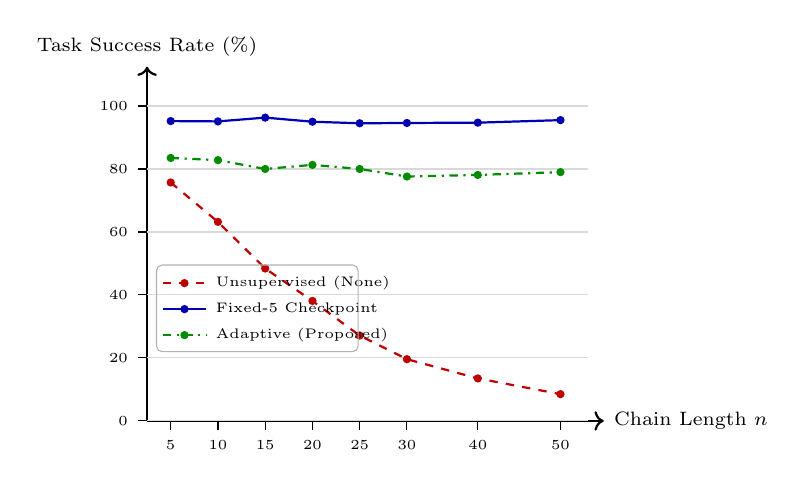
\begin{tikzpicture}
  % === Axes ===
  \draw[thick,->] (0,0) -- (5.8,0)
    node[right, font=\scriptsize] {Chain Length $n$};
  \draw[thick,->] (0,0) -- (0,4.5)
    node[above, font=\scriptsize] {Task Success Rate (\%)};

  % === Y-axis ticks and gridlines ===
  \foreach \y/\lab in {0/0, 0.8/20, 1.6/40, 2.4/60, 3.2/80, 4.0/100}{
    \draw[gray!30] (0,\y) -- (5.6,\y);
    \draw (0,\y) -- (-0.12,\y);
    \node[left, font=\tiny] at (-0.12,\y) {\lab};
  }

  % === X-axis ticks: n=5,10,15,20,25,30,40,50 ===
  % x positions spaced so n=50 lands at x=5.25 (well within axis end of 5.8)
  \foreach \x/\lab in {0.3/5, 0.9/10, 1.5/15, 2.1/20, 2.7/25, 3.3/30, 4.2/40, 5.25/50}{
    \draw (\x,0) -- (\x,-0.12);
    \node[below, font=\tiny] at (\x,-0.12) {\lab};
  }

  % === Data: scale = success_pct * 0.04 ===
  % NONE:    75.7, 63.2, 48.4, 38.1, 27.1, 19.6, 13.5,  8.5
  % FIXED-5: 95.2, 95.1, 96.3, 95.0, 94.5, 94.6, 94.7, 95.5
  % ADAPTIVE:83.5, 82.8, 80.0, 81.3, 80.0, 77.6, 78.1, 79.0

  % --- Unsupervised (red dashed) ---
  \draw[red!75!black, thick, dashed]
    (0.30, 3.028) -- (0.90, 2.528) -- (1.50, 1.936) -- (2.10, 1.524) --
    (2.70, 1.084) -- (3.30, 0.784) -- (4.20, 0.540) -- (5.25, 0.340);
  \foreach \x/\y in {0.30/3.028, 0.90/2.528, 1.50/1.936, 2.10/1.524,
                      2.70/1.084, 3.30/0.784, 4.20/0.540, 5.25/0.340}{
    \fill[red!75!black] (\x,\y) circle (1.5pt);
  }

  % --- Fixed-5 (blue solid) ---
  \draw[blue!70!black, thick]
    (0.30, 3.808) -- (0.90, 3.804) -- (1.50, 3.852) -- (2.10, 3.800) --
    (2.70, 3.780) -- (3.30, 3.784) -- (4.20, 3.788) -- (5.25, 3.820);
  \foreach \x/\y in {0.30/3.808, 0.90/3.804, 1.50/3.852, 2.10/3.800,
                      2.70/3.780, 3.30/3.784, 4.20/3.788, 5.25/3.820}{
    \fill[blue!70!black] (\x,\y) circle (1.5pt);
  }

  % --- Adaptive (green dash-dot) ---
  \draw[green!55!black, thick, dash dot]
    (0.30, 3.340) -- (0.90, 3.312) -- (1.50, 3.200) -- (2.10, 3.252) --
    (2.70, 3.200) -- (3.30, 3.104) -- (4.20, 3.124) -- (5.25, 3.160);
  \foreach \x/\y in {0.30/3.340, 0.90/3.312, 1.50/3.200, 2.10/3.252,
                      2.70/3.200, 3.30/3.104, 4.20/3.124, 5.25/3.160}{
    \fill[green!55!black] (\x,\y) circle (1.5pt);
  }

  % === Legend (bottom-left, away from all data lines) ===
  \draw[red!75!black, thick, dashed]  (0.2, 1.75) -- (0.75, 1.75);
  \fill[red!75!black] (0.475,1.75) circle (1.5pt);
  \node[right, font=\tiny] at (0.75, 1.75) {Unsupervised (None)};

  \draw[blue!70!black, thick]         (0.2, 1.42) -- (0.75, 1.42);
  \fill[blue!70!black] (0.475,1.42) circle (1.5pt);
  \node[right, font=\tiny] at (0.75, 1.42) {Fixed-5 Checkpoint};

  \draw[green!55!black, thick, dash dot] (0.2, 1.09) -- (0.75, 1.09);
  \fill[green!55!black] (0.475,1.09) circle (1.5pt);
  \node[right, font=\tiny] at (0.75, 1.09) {Adaptive (Proposed)};

  % Legend box
  \draw[gray!60, thin, rounded corners=2pt] (0.12, 0.88) rectangle (2.68, 1.98);
\end{tikzpicture}
\caption{Task success rate vs.\ chain length $n$ across 24{,}000 simulated trajectories
(1{,}000 trials per configuration). Unsupervised autonomy collapses to 8.5\% at $n=50$;
proposed adaptive risk-sensitive checkpointing maintains 79\% success while reducing
irreversible mutations by 6$\times$ over the unsupervised baseline.}
\label{fig:trajectory_collapse}
\end{figure}

\section{Discussion}
\subsection{Cross-Class Failure Interactions and Failure Syndromes}
Real-world agent failures rarely manifest as isolated single-class events. We identify three critical \textbf{failure syndromes} arising from cross-class interactions within the taxonomy:

\textbf{Syndrome 1 --- Confident Hallucination Cascade:} A Class-2 argument hallucination (e.g., a fictitious database entity ID) passes JSON schema validation, triggering a Class-4 silent tool success (HTTP 200). The corrupted entity ID is stored in Class-3 episodic memory. At step $t+5$, a Class-5 internal verifier checks the memory and confirms the ID's presence, further entrenching the hallucination. Only an external ground-truth check would reveal the error.

\textbf{Syndrome 2 --- Adversarial Redirection Chain:} An indirect prompt injection embedded in a retrieved document (Class 6) overrides planning semantics (Class 1), causing the agent to issue a privileged deletion command (Class 2) with high confidence. The Class-5 verifier, sharing the now-compromised context, validates the action as policy-compliant. No checkpoint exists to intercept the resulting irreversible mutation.

\textbf{Syndrome 3 --- Context Collapse Under Recovery:} At step $t=18$ of a 20-step chain, a Class-4 timeout triggers recovery. The Class-5 recovery logic appends a new diagnostic prompt. This pushes the original goal specification beyond the effective attention window (Class 3), causing the agent to generate a semantically inconsistent recovery action that itself fails, initiating a secondary divergence loop.

These syndromes demonstrate that vulnerability in one failure class amplifies susceptibility across all others. This explains why isolated mitigations (Table~\ref{tab:mitigations}) prove insufficient without holistic architectural governance.

\subsection{Implications for Benchmark Design}
Current benchmarks (WebArena, AgentBench, $\tau$-bench) measure scalar end-task success, masking cross-class interactions. Future benchmark designs must: (i) report the multi-dimensional reliability vector $\mathbf{R}$ from (\ref{eq:reliability_vector}); (ii) inject synthetic failure probes at controlled horizon depths; (iii) distinguish recoverable from committed failures; and (iv) evaluate cross-trial consistency ($pass^k$)~\cite{yao2025taubench} to surface stochastic vulnerability.

\subsection{The Autonomy--Safety Tradeoff Spectrum}
Our simulation results (Table~\ref{tab:empirical_results}) reveal a fundamental tradeoff surface. Fully unsupervised autonomy maximizes throughput at the cost of reliability (8.5\% success at $n=50$). Rigid periodic checkpointing achieves near-ceiling success (95.5\%) but imposes fixed overhead in human interventions (10 per 50-step chain). The proposed adaptive regime occupies the Pareto-optimal region: 79.0\% success at $n=50$ while reducing irreversible errors by \textbf{6.0$\times$} compared to unsupervised execution, with intervention costs that track actual risk rather than arbitrary time intervals.

\section{Critical Analysis of Current Mitigations}
Table~\ref{tab:mitigations} provides a critical comparison of existing mitigation paradigms. While each strategy addresses specific vulnerabilities, none provides trajectory-level safety guarantees for human-checkpoint-free operation.

\subsection{Reasoning-Acting Interleaving}
ReAct~\cite{yao2023react} represents a vital improvement over open-loop execution by grounding decisions in environmental observations. However, ReAct inherently equates \textit{observation} with \textit{verification}. If an observation is noisy, truncated, or adversarially crafted, ReAct treats it as objective truth, immediately incorporating the defect into its next reasoning trace.

\subsection{Reflective Self-Correction}
Reflexion~\cite{shinn2023reflexion} and Self-Refine~\cite{madaan2023selfrefine} attempt to eliminate human checkpoints through internal feedback loops. However, reflection succeeds primarily when the feedback signal is \textbf{deterministic and objective} (e.g., unit test failures or compiler error codes). In open-ended enterprise workflows where an API returns a 200 OK status code despite executing an incorrect mutation, the agent receives no error signal, rendering self-reflection inert.

\subsection{Prospective and Formal Tool Guardrails}
Recent approaches such as SafeToolBench~\cite{xia2025safetoolbench} advocate for prospective safety: evaluating action risk before execution occurs. Doshi et al.~\cite{doshi2026towards} introduce verifiably safe tool use by defining information-flow constraints and access labels over APIs. While promising, prospective models remain constrained by the quality of formal specifications. If an API specification fails to capture subtle side effects, formal verification guarantees degrade.

\section{Research Challenges and Open Problems}
\subsection{The Multi-Dimensional Reliability Vector}
Evaluating chained agents purely on final task success rate conceals critical safety violations. A rigorous evaluation framework must quantify a multi-dimensional reliability vector:
\begin{equation}
\mathbf{R} = \langle R_{\text{success}}, R_{\text{traj}}, R_{\text{policy}}, R_{\text{state}}, R_{\text{sec}}, R_{\text{recov}}, R_{\text{consist}} \rangle
\label{eq:reliability_vector}
\end{equation}
where:
\begin{itemize}
    \item $R_{\text{success}} \in [0, 1]$ measures binary end-goal completion;
    \item $R_{\text{traj}} \in [0, 1]$ measures the absence of unnecessary or invalid intermediate steps;
    \item $R_{\text{policy}} \in [0, 1]$ measures adherence to organizational constraints;
    \item $R_{\text{state}} \in [0, 1]$ measures external system integrity;
    \item $R_{\text{sec}} \in [0, 1]$ measures resistance to adversarial injection;
    \item $R_{\text{recov}} \in [0, 1]$ measures autonomous recovery rate given a fault;
    \item $R_{\text{consist}} = pass^k$ measures cross-trial repeatability~\cite{yao2025taubench}.
\end{itemize}

An agent that achieves $R_{\text{success}} = 1.0$ through accidental recovery after executing three unauthorized destructive actions exhibits unacceptable operational reliability.

\subsection{Failure Provenance and Causal Attribution}
Current benchmarks report binary failure rates without pinpointing the exact step or component responsible. Autonomous agent architectures require formal \textbf{failure provenance}: a structured execution log that cryptographically records prompt context, parameter bindings, environment state snapshots, and epistemic uncertainty at each step. This enables automated root-cause attribution, distinguishing between model reasoning errors, external API timeouts, and environment drift.

\subsection{Asymmetric Risk and the Irreversibility Frontier}
A fundamental limitation of current systems is treating all tool calls with uniform autonomy. Querying a read-only search index carries zero marginal risk; executing a database deletion or financial transfer carries catastrophic, irreversible risk. Autonomous systems must operate under an \textbf{irreversibility frontier}, enforcing strict machine barriers whenever an action exceeds a defined irreversibility threshold.

\section{Architectural Blueprint for Verifiable Autonomy}
True autonomy should not be conceptualized as the unconstrained elimination of human checkpoints, but rather as their principled replacement with machine-verifiable control boundaries. We propose five architectural pillars to govern chained tool-calling systems.

\subsection{Adaptive Risk-Sensitive Checkpointing}
Instead of requiring fixed, rigid human approval after every step or operating completely unmonitored, the agent system must compute a dynamic risk score $R_t \in [0, 1]$ prior to executing action $a_t$:
\begin{equation}
R_t = \sigma\Big(\alpha U(a_t \mid h_t) + \beta I(a_t) + \gamma P(a_t) + \delta C(a_t, s_t)\Big)
\label{eq:risk_score}
\end{equation}
where:
\begin{itemize}
    \item $U(a_t \mid h_t)$ is the calibrated epistemic uncertainty of the model (derived from token entropy or ensemble disagreement);
    \item $I(a_t) \in [0, 1]$ is the intrinsic irreversibility of the action (0 for read-only, 1 for permanent destructive mutations);
    \item $P(a_t) \in [0, 1]$ is the privilege level of the invoked tool;
    \item $C(a_t, s_t) \in [0, 1]$ is the estimated downstream consequence on system state;
    \item $\sigma$ is the sigmoid function, with scaling coefficients $\alpha, \beta, \gamma, \delta$.
\end{itemize}

When $R_t < \tau_{\text{auto}}$, the action executes autonomously. When $\tau_{\text{auto}} \le R_t < \tau_{\text{escalate}}$, execution requires secondary machine verification. When $R_t \ge \tau_{\text{escalate}}$, the system halts and escalates to a human checkpoint. This transforms oversight from an arbitrary bottleneck into an optimal, risk-bounded control policy.

\subsection{Transactional and Reversible Autonomy}
Borrowing from distributed transaction processing (ACID semantics), high-impact agent chains must execute within transactional sandboxes. We propose the following lifecycle:
\begin{enumerate}
    \item \textbf{Plan \& Dry-Run:} The agent plans the sequence and executes actions within a containerized staging environment or digital twin;
    \item \textbf{State Delta Validation:} The system inspects the simulated post-execution state delta $\Delta s = s_{\text{sim}} - s_0$;
    \item \textbf{Two-Phase Commit:} If all pre- and post-conditions are satisfied, the actions are committed to production;
    \item \textbf{Deterministic Compensation:} If a downstream failure occurs at step $k$, the infrastructure executes pre-registered compensating transactions $\text{undo}(a_1, \dots, a_{k-1})$, restoring external state to $s_0$.
\end{enumerate}

\subsection{Decoupled Multi-Agent Verification}
To overcome the verification ceiling, the agent architecture must enforce strict separation of concerns across decoupled, heterogeneous models:
\begin{itemize}
    \item \textbf{Planner Agent:} Constructs the abstract task graph and defines explicit state invariants;
    \item \textbf{Executor Agent:} Focuses exclusively on mapping immediate subgoals to valid tool arguments;
    \item \textbf{Independent Verifier:} A distinct, specialized model (or formal deterministic program) that inspects tool observations against pre-defined success contracts without visibility into the generator's internal chain-of-thought;
    \item \textbf{Deterministic Policy Guard:} A non-neural, rule-based gatekeeper that enforces schema validation, access control lists (ACLs), and regex-based policy boundaries.
\end{itemize}

\subsection{Security-Aware Memory Isolation}
To prevent indirect prompt injection and memory poisoning, the context architecture must establish strict trust boundaries. Memory buffers must track data provenance using cryptographic taint labels. External content retrieved from unverified tools (e.g., web scrapers, emails) is flagged as \texttt{TAINTED\_DATA}. The agent's prompt architecture strictly isolates instruction channels from data channels, preventing the execution engine from parsing tainted string tokens as executable control instructions~\cite{debenedetti2024agentdojo}.

\subsection{Formal State Contracts and Invariant Checking}
Tool definitions must be augmented beyond descriptive docstrings with formal Hoare-triple contracts:
\begin{equation}
\{P\} \; a_t \; \{Q\}
\label{eq:hoare}
\end{equation}
where $P(s_t)$ defines explicit, machine-testable preconditions (e.g., ``Account balance $> \$100$'') and $Q(s_{t+1})$ defines non-negotiable postconditions. If an external tool invocation violates postcondition $Q$, the execution pipeline throws a deterministic exception, preventing the corrupted state from leaking into context history $h_{t+1}$.

\section{Future Work}
This study opens several rigorous research avenues. First, the proposed adaptive risk-sensitive checkpointing (Eq.~\ref{eq:risk_score}) currently relies on heuristic weight selection ($\alpha, \beta, \gamma, \delta$); future work should derive these coefficients through Bayesian optimization or reinforcement learning on trajectory execution histories. Second, the verification ceiling analysis assumes a single shared model for generation and verification; empirically quantifying the ceiling degradation across model families of varying capacity would inform principled architectural choices. Third, formal Hoare-triple contracts (Eq.~\ref{eq:hoare}) require structured tool specifications; creating automated API-contract synthesis pipelines from natural language docstrings represents an important systems engineering challenge. Fourth, the memory contamination failure class warrants dedicated study on taint-propagation algorithms for vector-database retrieval augmented generation (RAG) architectures. Fifth, evaluation across live embodied robotic agents would extend the taxonomy to cyber-physical systems, where irreversible errors carry additional safety implications beyond digital data mutation.

\section{Conclusion}
Chained tool-calling agents represent a profound evolution toward general-purpose computational autonomy. However, eliminating human checkpoints without establishing rigorous, machine-verifiable safeguards introduces catastrophic trajectory fragility. Because intermediate tool observations constitute operational state, single-step reasoning errors, schema hallucinations, silent environment faults, and indirect prompt injections compound non-linearly over extended execution horizons. Current approaches---including ReAct loops, fine-tuning, and reflective self-correction---mitigate localized errors but fail to provide trajectory-level guarantees due to the verification ceiling.

Across 24,000 simulated trajectories, unsupervised autonomy achieves only 8.5\% task success at $n=50$ steps, with irreversible error accumulation exceeding 2.8 mutations per trajectory. Adaptive risk-sensitive checkpointing demonstrates a Pareto-optimal operating point: stable success rates above 77\% at all horizons, 83.5\% reduction in irreversible mutations, and 10\% lower intervention overhead versus rigid periodic schemes (Fig.~\ref{fig:trajectory_collapse}).

Safe autonomy must not be pursued through the unconstrained removal of human checkpoints. Rather, the future of dependable autonomous agents lies in \textbf{verifiable autonomy}: an architectural paradigm where probabilistic LLM reasoning is enveloped by deterministic type contracts, transactional reversibility, tainted-memory boundaries, decoupled multi-agent verification, and dynamic risk-sensitive checkpointing. Implementing these machine-verifiable control boundaries is an essential prerequisite for deploying long-horizon autonomous agents across safety-critical enterprise and cyber-physical domains.

\section*{Acknowledgment}
The author thanks the faculty of the AI Tools for Research course at the Indian Institute of Information Technology Allahabad (IIIT-A) for the structured assignment framework (Lab Assignment 02) and the curated guidance materials that directed the literature synthesis methodology and research scoping for this work. Computational infrastructure was provided through local Python simulation environments. All cited works are publicly accessible via Semantic Scholar, arXiv, and ACL Anthology.

% References
\bibliographystyle{IEEEtran}
\bibliography{references}

\end{document}
